%==============================================================
This chapter describes the MCS-4 Chip Set and System Architecture.
%==============================================================
\section{Introduction}
This book aims to logically design the Intel 4004 (CPU), the centerpiece of the MCS-4 system, the world's first microcomputer, using Verilog HDL, implement it on an FPGA, and ultimately recreate the historic Busicom 141-PF calculator. In this chapter, we begin with a detailed explanation of the overall architecture of the MCS-4 system, starting with the 4004.\cite{MCS4HardwareManual}

%==============================================================
\section{Getting Comfortable with 4 Bits}
Since the 4004 is a 4-bit CPU, data is fundamentally handled in 4-bit units. Accordingly, data addresses are also assigned in 4-bit increments. Those of you who grew up with microcomputers might be more familiar with 8-bit data and addressing, so working with 4-bit units might feel a bit strange at first. But I encourage you to embrace that sensation-find enjoyment in the unfamiliar. Note that instruction codes of 4004 are 8-bit, so their addresses are assigned in 8-bit units.\\

In the world of data, 8 bits make up a ``byte'',  and likewise, 4 bits are referred to as a ``nibble''. This chapter uses the term nibble frequently, so take some time to get comfortable with it.\\

Incidentally, one theory behind the term ``byte'' is that it's a playful twist on the word ``bite'', as in a bite of data. The word ``nibble'',  fittingly, means ``to take a small bite''. To add another layer of trivia: ``data'' is the plural form of ``datum'', which comes from the Latin word ``dare'', meaning ``to give''. In short, when something is given to you, you should chew or nibble thoughtfully. \\

Just don't expect much excitement from the word ``bit''—it's short for ``binary digit'', and that etymology is as dry as it sounds.\\

While a byte is commonly understood today to be 8 bits, that hasn't always been the case. Historically, ``byte'' simply referred to the number of bits needed to encode a character, ranging anywhere from 5 to 12 bits (according to Wikipedia). These days, 8 bits are generally referred to as a byte, but if you want to be exact, the proper term for an 8-bit unit is ``octet''. Similarly, a ``nibble'' precisely represents 4 bits.

%==============================================================
\section{MCS-4 Chip Set}
To build a 4-bit microcomputer system, four types of chips are used: the 4004 (CPU), 4001 (ROM), 4002 (RAM), and 4003 (Shift Register). Typically, only one 4004 exists within the system, while multiple units of the 4001, 4002, and 4003 are used depending on the configuration. An overview of their specifications is shown in Table \ref{tb:MCS4CHIPSETOVERVIEW}.\\

The 4001 functions as a mask ROM with input/output ports, the 4002 serves as RAM with output ports, the 4003 is a shift register for expanding output ports, and the 4004 is the 4-bit CPU. There are two variants of the 4002 RAM chip: the 4002-1 and the 4002-2. These are provided to handle differences in how chip numbers are assigned within RAM banks.

%----------------------------------------------------
\begin{table}[htbp]
\centering
\begin{tabular}{|l|l|l|p{8cm}|}
\hline
\rowcolor{LightPurple}
\textbf{Type} & \textbf{Name} & \textbf{Item} & \textbf{Details} \\
\hline
CPU & 4004 & Function & 4-bit CPU \\
\cline{3-4}
     &      & Instruction Set & 46 instructions \\
\cline{3-4}
     &      & Instruction Length & 8-bit or 16-bit \\
\cline{3-4}
     &      & Memory Space & ROM: 4KB; RAM: 1280 nibbles (direct), 2560 nibbles (with external circuits) \\
\cline{3-4}
     &      & Operating Frequency & Up to 740.7KHz (1.35 µs) \\
\cline{3-4}
     &      & Instruction Cycle & Minimum 10.8 µs \\
\cline{3-4}
     &      & Package & 16-pin DIP \\
\hline
ROM & 4001 & Function & Mask ROM and I/O port \\
\cline{3-4}
     &      & ROM Capacity & 256 words × 8 bits (256 bytes per chip) \\
\cline{3-4}
     &      & Chips per System & Up to 16 chips (chip number set via metal options) \\
\cline{3-4}
     &      & I/O Ports & One 4-bit port per chip (I/O direction and pull-up/down set via metal options) \\
\cline{3-4}
     &      & Package & 16-pin DIP \\
\hline
RAM & 4002 & Function & RAM and output port \\
\cline{3-4}
     &      & RAM Capacity & 4 registers per chip; 16 nibbles (main) + 4 nibbles (status) per register; total 320 bits per chip \\
\cline{3-4}
     &      & Banks per System & Max 4 banks (direct); Max 8 banks (external circuit) \\
\cline{3-4}
     &      & Chips per Bank & Max 4 chips per bank; 4002-1 for chips \#0 and \#1, 4002-2 for \#2 and \#3 \\
\cline{3-4}
     &      & Output Port & One 4-bit output port per chip \\
\cline{3-4}
     &      & Package & 16-pin DIP \\
\hline
Shifter & 4003 & Function & 10-bit shift register (serial to parallel conversion) \\
\cline{3-4}
     &       & Cascade Capability & Supported \\
\cline{3-4}
     &       & Reset & Power-on reset clears shift register \\
\cline{3-4}
     &       & Output Control & OE=1: outputs data; OE=0: outputs all zero \\
\cline{3-4}
     &       & Package & 16-pin DIP \\
\hline
\end{tabular}
\caption{Overview of MCS-4 Chip Set Specifications}
\label{tb:MCS4CHIPSETOVERVIEW}
\end{table}
%----------------------------------------------------

%==============================================================
\section{4004 CPU}
%----------------------------------------------------
\subsection{Functional Overview of the 4004 CPU}
The 4004 is a 4-bit CPU core at the heart of the MCS-4 system. It fetches instructions from ROM, decodes the instruction code, and executes operations accordingly.

Each instruction cycle consists of 8 clock cycles, during which the CPU transitions sequentially through eight internal states: A1, A2, A3, M1, M2, X1, X2, and X3.

With a maximum operating frequency of 740~kHz, each instruction cycle lasts approximately 10.8~µs (minimum). Naturally, the 4004 does not utilize pipelined control; instruction fetch, decode, and execution are processed one at a time in strict sequence.

Detailed timing of instruction execution and behavior of individual instructions will be described later.
%----------------------------------------------------
\subsection{Pin layout and Signal Functions of the 4004 CPU}
Figure \ref{fig:PINOUT4004} shows the pin layout and the signal functions of the 4004 CPU. The role of each signal is described below:

\begin{enumerate}[\textbf{(\arabic*)}]
  \item \textbf{$\Phi$1, $\Phi$2 (Clock Inputs):}  
    The internal logic employs dynamic latch circuits, requiring a two-phase clock input. In this documentation’s redesign of the MCS-4, all circuits use D flip-flops and a single-phase clock.

  \item \textbf{$\overline{\text{RESET}}$ (Reset Input):} 
    A signal used to reset the internal logic of the CPU.

  \item \textbf{D0--D3 (Data Bus):} 
    A 4-bit bidirectional data bus. The 4004 does not have a separate address bus; address information is also carried via the data bus, with time-division multiplexing used to exchange address and data between the CPU and ROM/RAM.

  \item \textbf{$\overline{\text{SYNC}}$ (Synchronization Signal Output):}  
    This signal ensures synchronized operation among the CPU, ROM, and RAM so their internal states transition simultaneously. Each chip monitors the SYNC signal from the CPU to align its internal state progression.

  \item \textbf{$\overline{\text{CM-ROM}}$ (ROM Command Control Output):}  
    A signal indicating how the ROM should interpret the data on the bus during each internal state.

  \item \textbf{$\overline{\text{CM-RAM0}}$ to $\overline{\text{CM-RAM3}}$ (RAM Command Control Outputs):}  
    Signals indicating how each RAM chip should interpret the data bus contents during each internal state.

  \item \textbf{TEST (Conditional Branch Input Signal):}  
    An input used to evaluate branch conditions in the JCN (Jump Conditional) instruction.
\end{enumerate}

%----------------------------------
\begin{figure}
    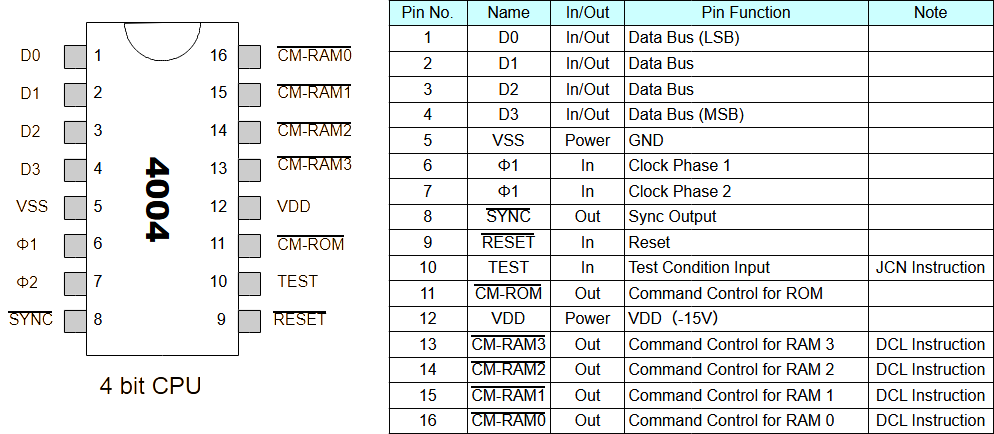
\includegraphics[width=1.0\columnwidth]{./Figure/Pinout4004.png}
    \caption{Pinout of 4004 CPU chip}
    \label{fig:PINOUT4004}
\end{figure}
%----------------------------------

%==============================================================
\section{4001 ROM}
%----------------------------------------------------
\subsection{Functional Overview of the 4001 ROM}
The 4001 is a ROM designed to store programs for the MCS-4 system. Each ROM chip has a capacity of 256 words by 8 bits. Additionally, the 4001 includes input/output port functionality.

The 4004 CPU can be directly connected to up to 16 ROM chips (a total of 4 KB). It is also possible to extend this capacity further with additional external circuitry.

This is a mask ROM: the ROM code must be submitted upon ordering, and the ROM pattern is permanently burned into the chip during manufacturing.

%----------------------------------------------------
\subsection{Pin layout and Signal Functions of the 4001 ROM}
Figure \ref{fig:PINOUT4001} shows the pin layout and the signal functions of the 4001 ROM. The role of each signal is described below:

\begin{enumerate}[\textbf{(\arabic*)}]
  \item \textbf{$\Phi$1, $\Phi$2 (Clock Inputs):}  
    Two-phase clock inputs. The same clock used by the 4004 CPU is applied here.

  \item \textbf{$\overline{\text{RESET}}$ (Reset Input):}  
    A signal used to reset the internal logic.

  \item \textbf{D0--D3 (Data Bus):}  
    A 4-bit bidirectional data bus.

  \item \textbf{$\overline{\text{SYNC}}$ (Synchronization Input):}  
    An input signal used to synchronize operation with the CPU.

  \item \textbf{$\overline{\text{CM}}$ (Command Control Input):}  
    This terminal connects to the $\overline{\text{CM-ROM}}$ signal generated by the CPU. The ROM interprets the data on the data bus based on the internal state in which the $\overline{\text{CM}}$ signal is asserted.

  \item \textbf{IO0--IO3 (Input/Output Ports):}  
    A 4-bit I/O port. Unlike modern microcontrollers that configure port direction and pull-up/down resistors via software registers, the 4001's configuration is fixed during chip fabrication via metal options.

  \item \textbf{$\overline{\text{CL}}$ (Register Clear Input for Output Ports):}  
    An input signal used to clear the output port's data register (flip-flops) to zero.
\end{enumerate}

%----------------------------------
\begin{figure}
    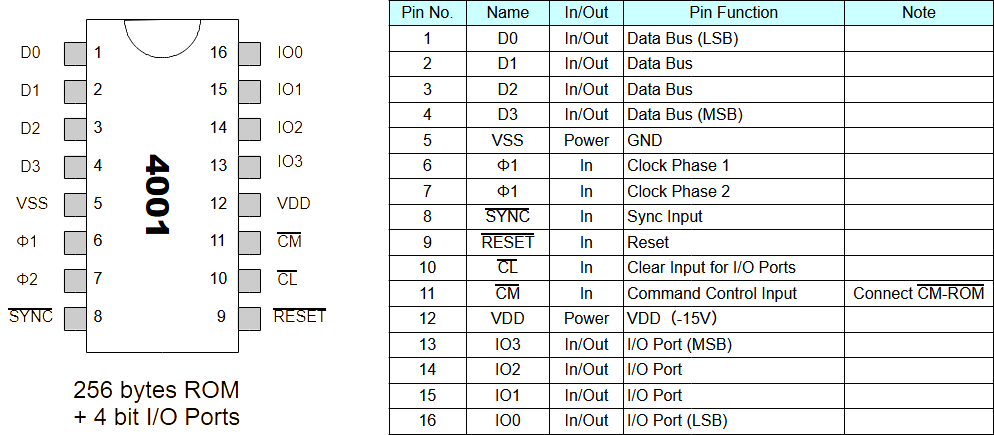
\includegraphics[width=1.0\columnwidth]{./Figure/Pinout4001.png}
    \caption{Pinout of 4001 ROM chip}
    \label{fig:PINOUT4001}
\end{figure}
%----------------------------------

%----------------------------------
\subsection{Internal Architecture of the 4001 ROM}
The internal structure of the 4001 is shown in Figure~3.

Eeach 4001 chip contains ROM memory organized into 256 words by 8 bits.

When the CPU accesses data stored in ROM (the access method will be explained later), a single word (8 bits) is read over a 4-bit data bus. The ROM outputs the upper 4 bits (OPR: operation code) and the lower 4 bits (OPA: modifier) sequentially.

Additionally, the chip includes a 4-bit input/output port. The configuration of each port (input/output direction, presence of pull-up/pull-down resistors) is specified at the time of chip fabrication using metal options (M1 through M10), as illustrated in Figure~3(b).

The CPU provides dedicated instructions to read from or write to these I/O ports.

When placing an order for the 4001 chip, users must submit both the ROM pattern and their desired metal option configuration for the I/O ports.

%----------------------------------
\begin{figure}
    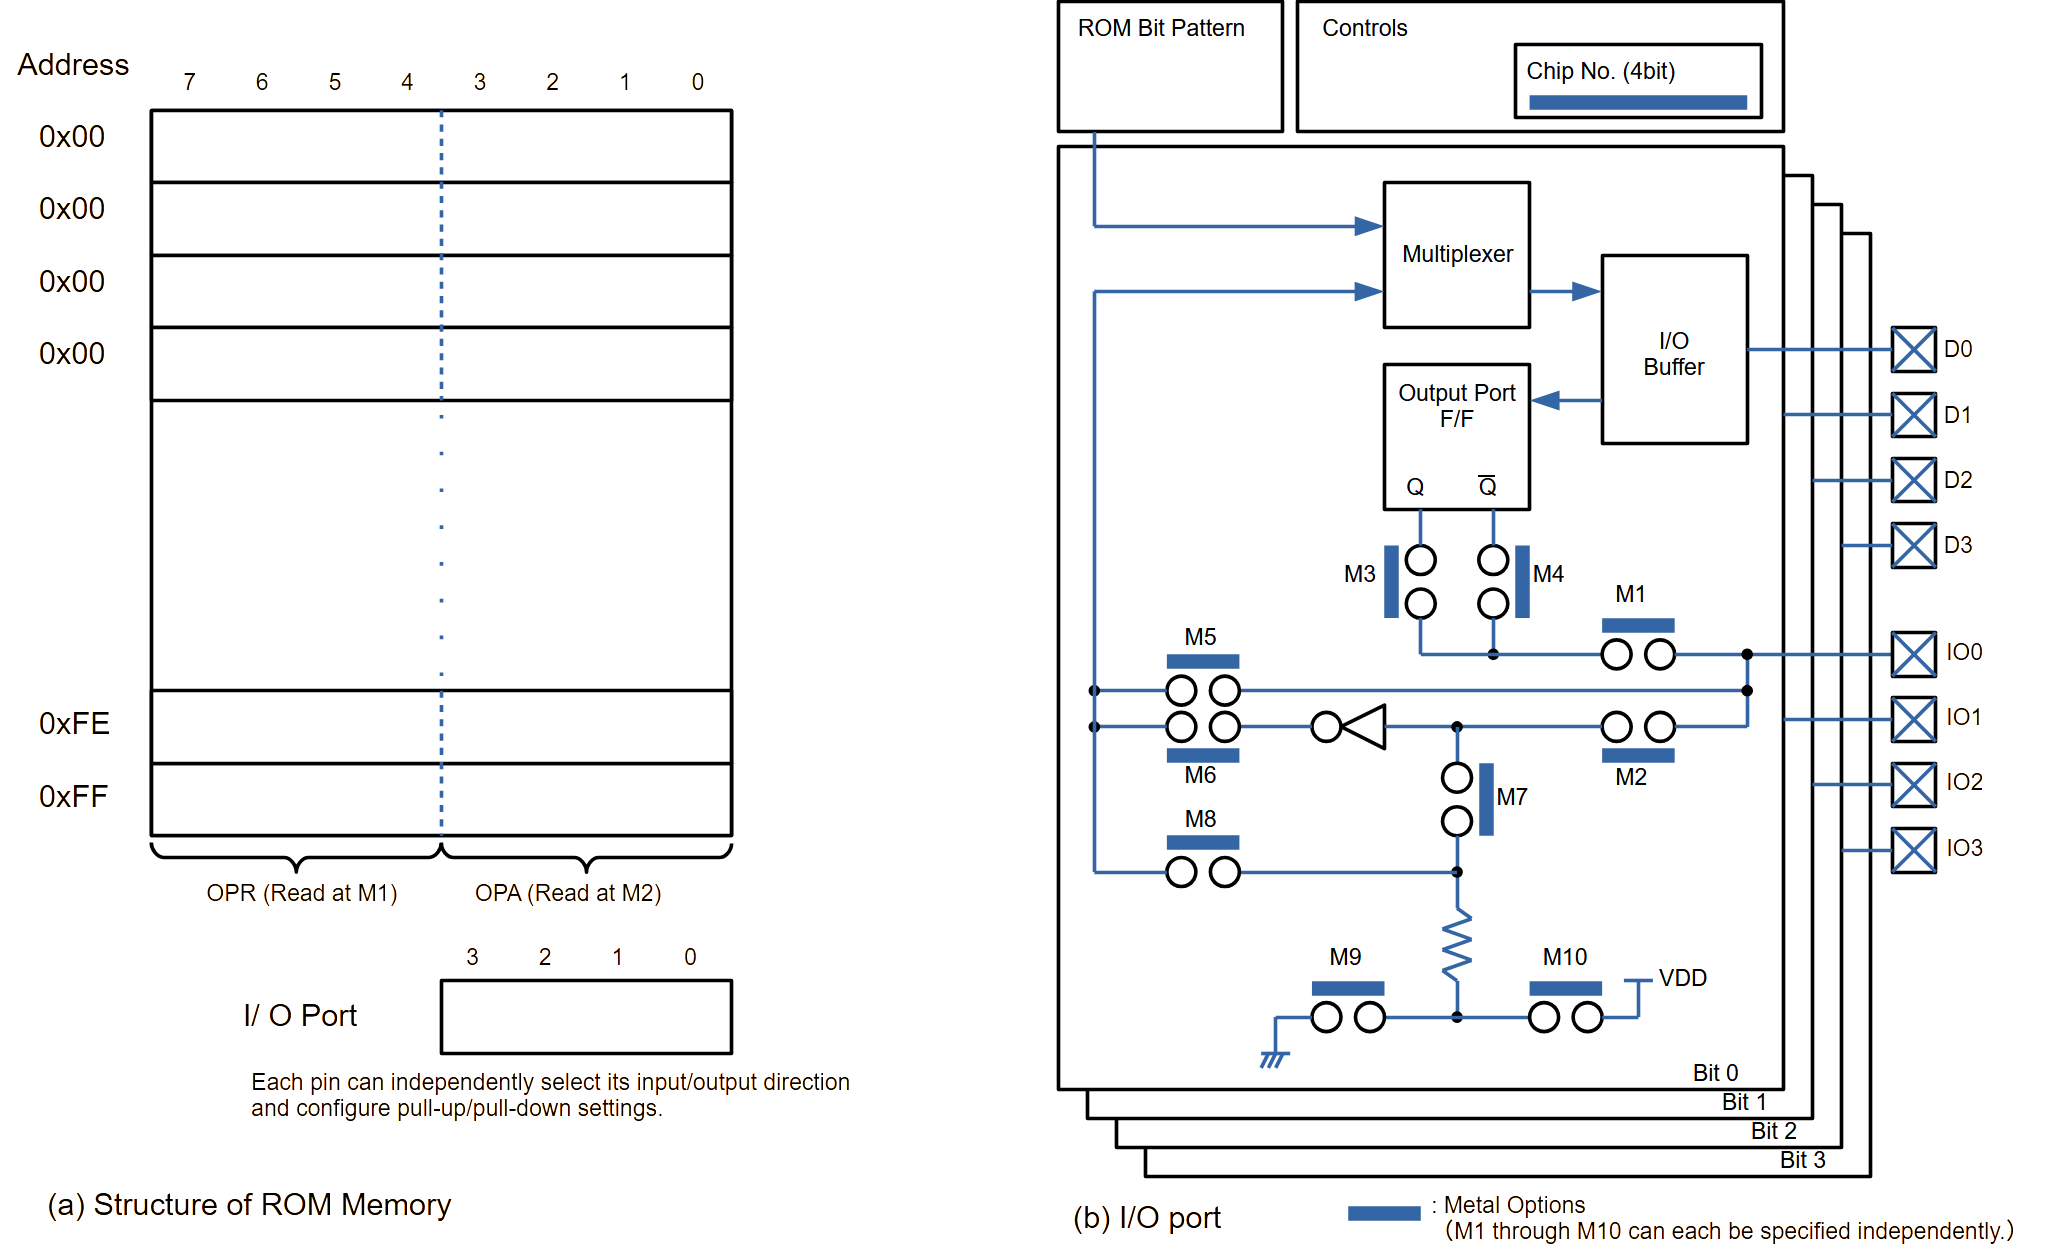
\includegraphics[width=1.0\columnwidth]{./Figure/Structure4001.png}
    \caption{Structure of 4001 ROM chip}
    \label{fig:STRUCTURE4001}
\end{figure}
%----------------------------------

%----------------------------------
\subsection{CPU Addressing of the 4001 ROM}
When the CPU accesses the 4001 ROM, it uses a 12-bit address space covering up to 4 KB. The upper 4 bits of the address serve as the chip number.

Each 4001 chip must be assigned a unique 4-bit chip number (ranging from 0 to 15), which is also specified as a metal option at the time of ordering.

%==============================================================
\section{4002 RAM}
%----------------------------------------------------
\subsection{Functional Overview of the 4002 RAM}
The 4002 is a RAM chip used for storing temporary data. Each 4002 chip contains 320 bits (80 nibbles) of RAM. While the capacity may seem peculiar, the reason behind it will be discussed later.

In addition, the 4002 also includes a 4-bit wide output port. Please note that the port direction is output-only.

From the CPU's perspective, the RAM chip group is organized hierarchically. The uppermost layer is called the \textit{bank}, and the subordinate layer consists of individual chips. The signals $\overline{\text{CM-RAM0}}$ to $\overline{\text{CM-RAM3}}$ correspond to the bank layer, and the RAM chips within the bank that receives an asserted $\overline{\text{CM-RAMx}}$ signal are accessed accordingly.

Beneath the bank layer is the chip layer, with four 4002 RAM chips comprising a single bank.

When connecting RAM directly to the CPU without external circuitry, $\overline{\text{CM-RAM0}}$ to $\overline{\text{CM-RAM3}}$ are asserted using a one-hot method. In this configuration, the system supports up to four RAM banks, resulting in a total of 16 RAM chips (RAM capacity: 5120 bits = 1280 nibbles = 640 bytes).

If more than four RAM banks are desired within the system, the CPU can output encoded $\overline{\text{CM-RAM0}}$ to $\overline{\text{CM-RAM3}}$ signals. These signals are decoded externally to generate a corresponding set of one-hot $\overline{\text{CM-RAMx}}$ signals, each selecting a RAM bank. According to the CPU's instruction specifications, this encoding allows for a maximum of 8 selectable banks. In this extended configuration, the system accommodates up to 32 RAM chips (RAM capacity: 10,240 bits = 2560 nibbles = 1280 bytes).

%----------------------------------------------------
\subsection{Pin layout and Signal Functions of the 4002 RAM}
Figure \ref{fig:PINOUT4002} shows the pin layout and the signal functions of the 4002 RAM. The role of each signal is described below:

\begin{enumerate}[\textbf{(\arabic*)}]
  \item \textbf{$\Phi$1, $\Phi$2 (Clock Inputs):}  
    These are two-phase clock inputs. The same clock used by the 4004 CPU is applied.

  \item \textbf{$\overline{\text{RESET}}$ (Reset Input):}  
    A signal used to reset the internal logic of the RAM. While $\overline{\text{RESET}}$ is asserted, the internal counter scans the RAM cells and clears its contents. Therefore, $\overline{\text{RESET}}$ must remain asserted for at least 32 instruction cycles, equivalent to 256 clock cycles.

  \item \textbf{D0--D3 (Data Bus):}  
    A 4-bit bidirectional data bus.

  \item \textbf{$\overline{\text{SYNC}}$ (Synchronization Input):}  
    An input signal used to synchronize the operation of the RAM with the CPU.

  \item \textbf{$\overline{\text{CM}}$ (Command Control Input for RAM):}  
    This terminal connects to the $\overline{\text{CM-RAMx}}$ output from the CPU. The interpretation of data on the data bus depends on the internal state in which the $\overline{\text{CM}}$ signal is asserted.

  \item \textbf{O0--O3 (Output Port):}  
    A 4-bit output-only port.

  \item \textbf{P0 (Chip Select Condition Input):}  
    An input signal used to select the chip number of the 4002 RAM.
\end{enumerate}

%----------------------------------
\begin{figure}
    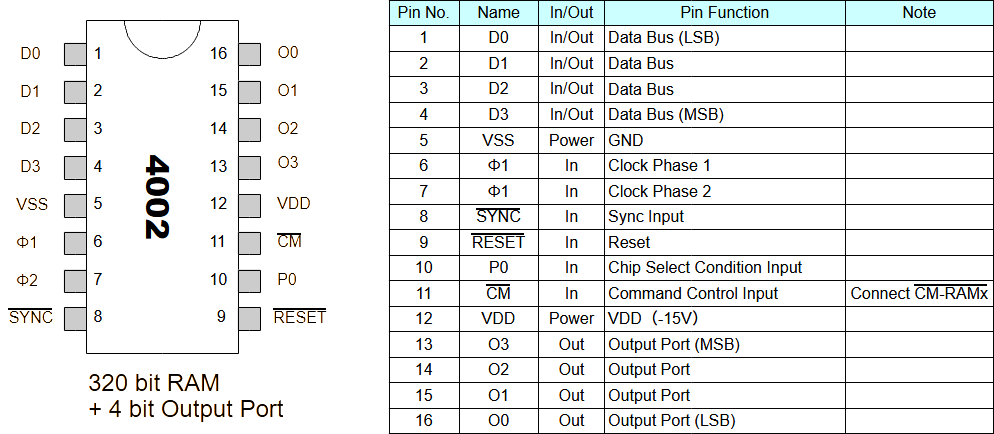
\includegraphics[width=1.0\columnwidth]{./Figure/Pinout4002.png}
    \caption{Pinout of 4002 RAM chip}
    \label{fig:PINOUT4002}
\end{figure}
%----------------------------------

%----------------------------------
\subsection{Internal Architecture of the 4002 RAM}
The internal structure of the 4002 RAM is shown in Figure \ref{fig:STRUCTURE4002}.

The 4002 RAM chip consists of four hierarchical blocks referred to as \textit{registers}. Each register contains 16 main memory characters (nibbles, 64 bits) and 4 status characters (nibbles, 16 bits). All are accessible for read and write operations via CPU instructions.

Since one register comprises a total of 80 bits of RAM, and there are four registers, a single 4002 chip holds 320 bits of RAM in total—equivalent to 80 nibbles or 40 bytes.

Within a single bank, the main memory character capacity reaches a maximum of 256 nibbles (128 bytes), while the status character capacity extends to 16 blocks, totaling 64 nibbles (32 bytes).

Remarkably, the RAM cells in the 4002 are implemented as dynamic memory. As such, periodic refresh is required. This refresh is performed automatically by an internal counter, which scans the RAM cells during idle periods within the instruction execution cycle (M1 and M2 states).

Additionally, the 4002 RAM includes a 4-bit output port. The CPU provides dedicated instructions for writing data to this port.

%----------------------------------
\begin{figure}
    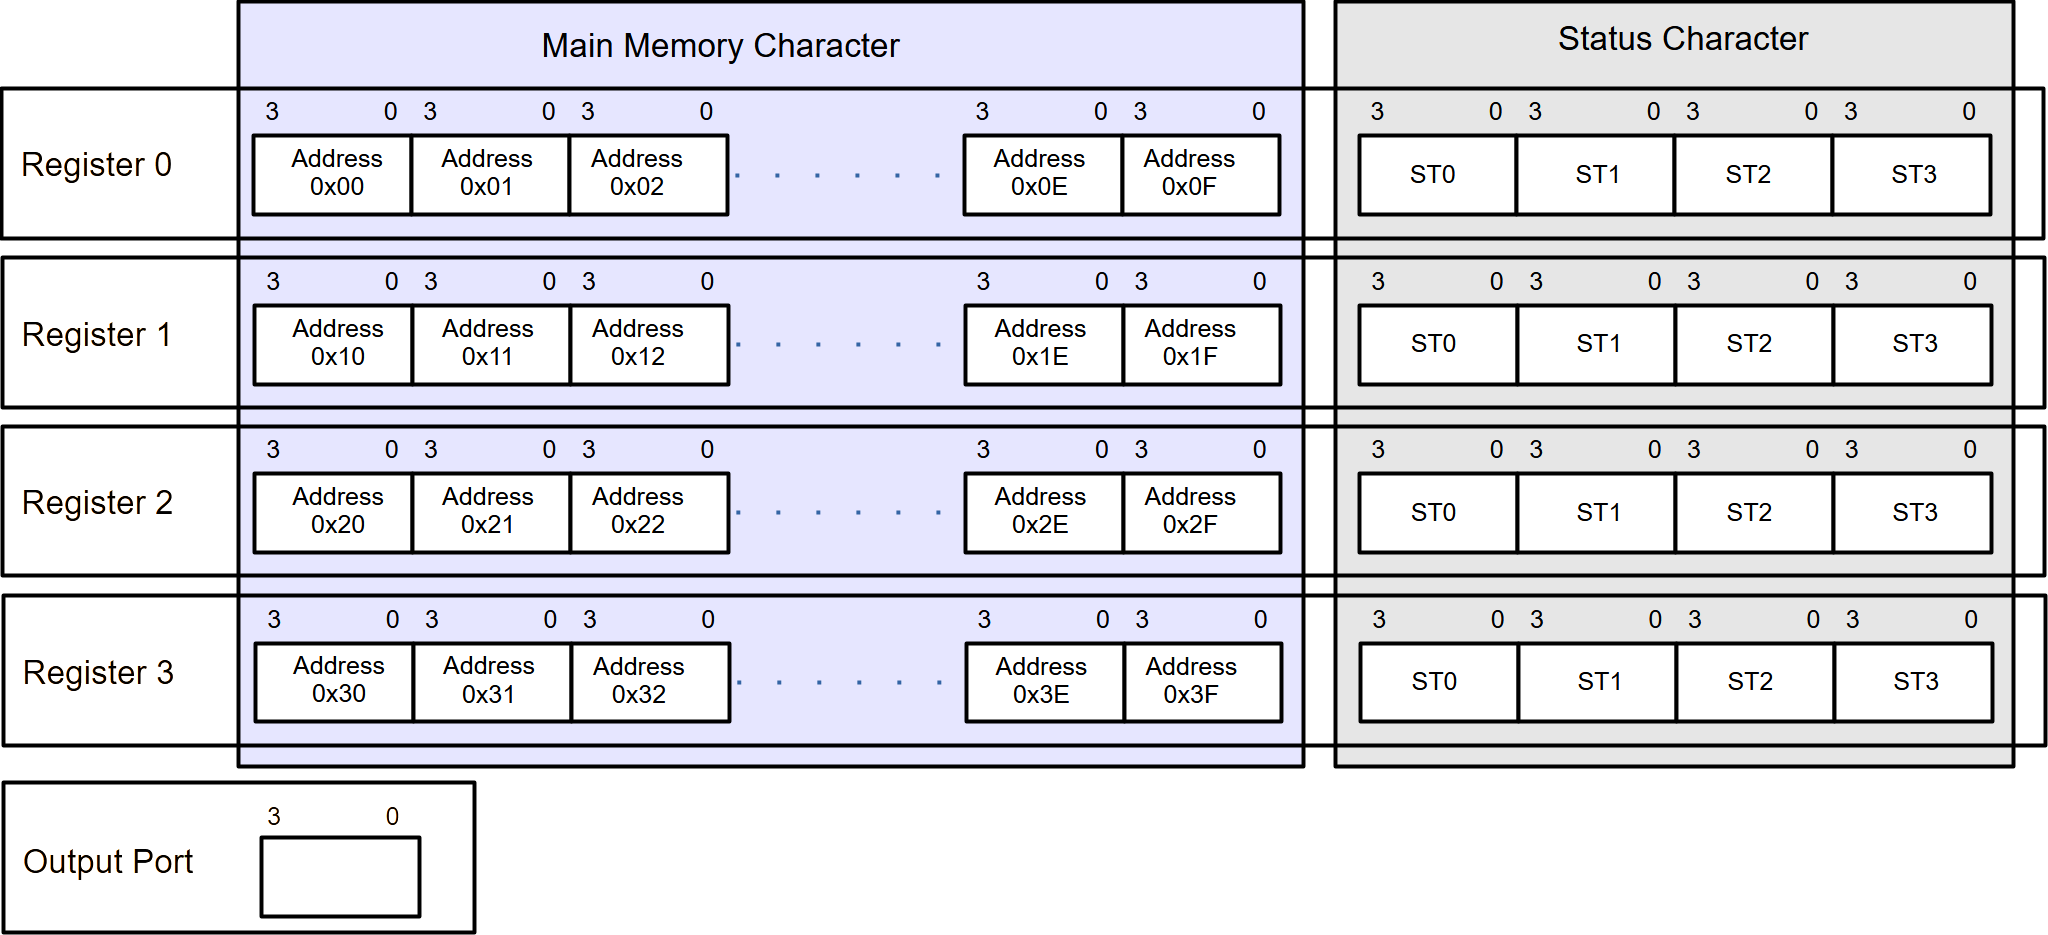
\includegraphics[width=1.0\columnwidth]{./Figure/Structure4002.png}
    \caption{Structure of 4002 RAM chip}
    \label{fig:STRUCTURE4002}
\end{figure}
%----------------------------------

%----------------------------------
\subsection{CPU Addressing of the 4002 RAM}

When addressing the 4002 RAM, the CPU specifies the following hierarchy: \textit{bank} (4 to 8 units), \textit{chip} (4 units), \textit{register} (4 units), and either \textit{main memory character} (16 units) or \textit{status character} (4 units).

The bank is selected using the $\overline{\text{CM-RAMx}}$ signal. Lower hierarchical levels—chip, register, and character—are specified using 8-bit address information sent from the CPU to the RAM (known as the SRC address, described later).

Chip numbers must be hardware-assigned to each RAM chip in the system. Since there are four chips per bank, a 2-bit identifier is required for chip selection. One of these bits is designated via input pin \texttt{P0}. As there is no additional terminal available for the second bit, chip selection is achieved by differentiating between two types of RAM chips—\texttt{4002-1} and \texttt{4002-2}—as described in Table \ref{tb:RAMCHIPSELECTION}.

%----------------------------------
\begin{table}[h]
\centering
\begin{tabular}{|p{2cm}|p{2cm}|p{2cm}|c|}
\hline
\rowcolor{LightPurple}
\textbf{4002 Chip Type} & \textbf{P0 Input Level} & \textbf{Chip No. within Bank} & \textbf{SRC Address Bits 7 and 6} \\
\hline
4002-1 & GND & 0 & Selected when bits = \texttt{00} \\
4002-1 & VDD & 1 & Selected when bits = \texttt{01} \\
4002-2 & GND & 2 & Selected when bits = \texttt{10} \\
4002-2 & VDD & 3 & Selected when bits = \texttt{11} \\
\hline
\end{tabular}
\caption{4002 RAM Chip Selection by P0 and SRC Address Bits}
\label{tb:RAMCHIPSELECTION}
\end{table}
%----------------------------------

%==============================================================
\section{4003 Shift Regieter}
%----------------------------------------------------
\subsection{Functional Overview of the 4003 Shift Register}
The 4003 is a 10-bit shift register IC designed to perform serial-to-parallel data conversion. It also supports cascade connections, allowing for significant expansion of system output ports.

The 4003 is typically connected to the output ports of the 4001 ROM or the 4002 RAM for practical use in the MCS-4 system.

%----------------------------------------------------
\subsection{Pin layout and Signal Functions of the 4003 Shift Register}
Figure \ref{fig:PINOUT4003} shows the pin layout and the signal functions of the 4003 Shift Register. The role of each signal is described below:

\begin{enumerate}[\textbf{(\arabic*)}]
  \item \textbf{CP (Clock Input):}  
    Clock signal for shift input. Data is shifted on the rising edge.

  \item \textbf{DATAIN (Serial Data Input):}  
    Serial data input signal to the shift register.

  \item \textbf{SERIALOUT (Serial Data Output):}  
    Serial data output signal from the shift register.

  \item \textbf{Q0--Q9 (Parallel Outputs):}  
    Parallel outputs of the 10-bit shift register.

  \item \textbf{OE (Output Enable):}  
    When OE = 1, the values stored in the shift register are output to Q0--Q9.  
    When OE = 0, Q0--Q9 output all zeros.
\end{enumerate}

%----------------------------------
\begin{figure}
    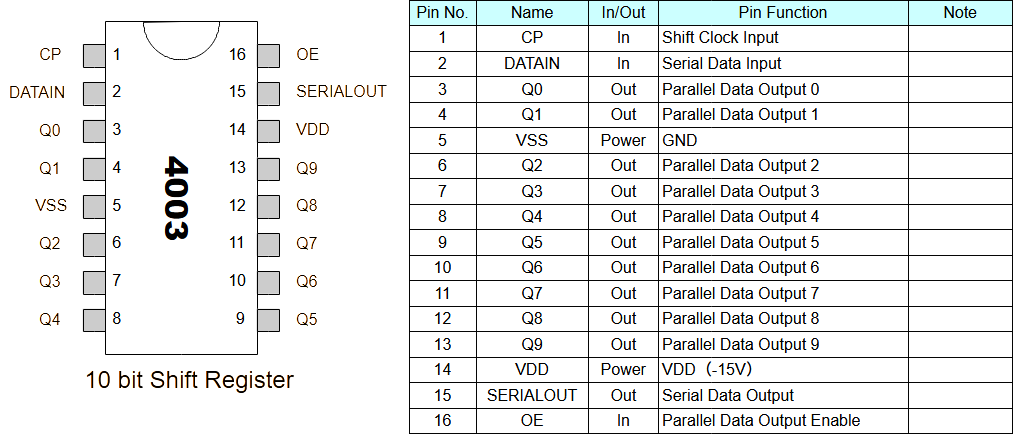
\includegraphics[width=1.0\columnwidth]{./Figure/Pinout4003.png}
    \caption{Pinout of 4003 Shift Regisster chip}
    \label{fig:PINOUT4003}
\end{figure}
%----------------------------------

%----------------------------------
\subsection{Internal Architecture of the 4003 Shift Register}

Figure \ref{fig:STRUCTURE4003} shows the internal configuration of the 4003, which implements a simple shift register.

The internal circuit of the CP clock input includes a delay line, allowing the serial data input signal \texttt{DATAIN} to change at the exact timing of the rising clock edge without requiring a setup time.

Similarly, the \texttt{SERIALOUT} signal also includes a delay circuit to ensure data hold time, thereby enabling cascade connections among multiple 4003 chips.

The shift register is cleared to zero via a power-on reset circuit.

%----------------------------------
\begin{figure}[H]
    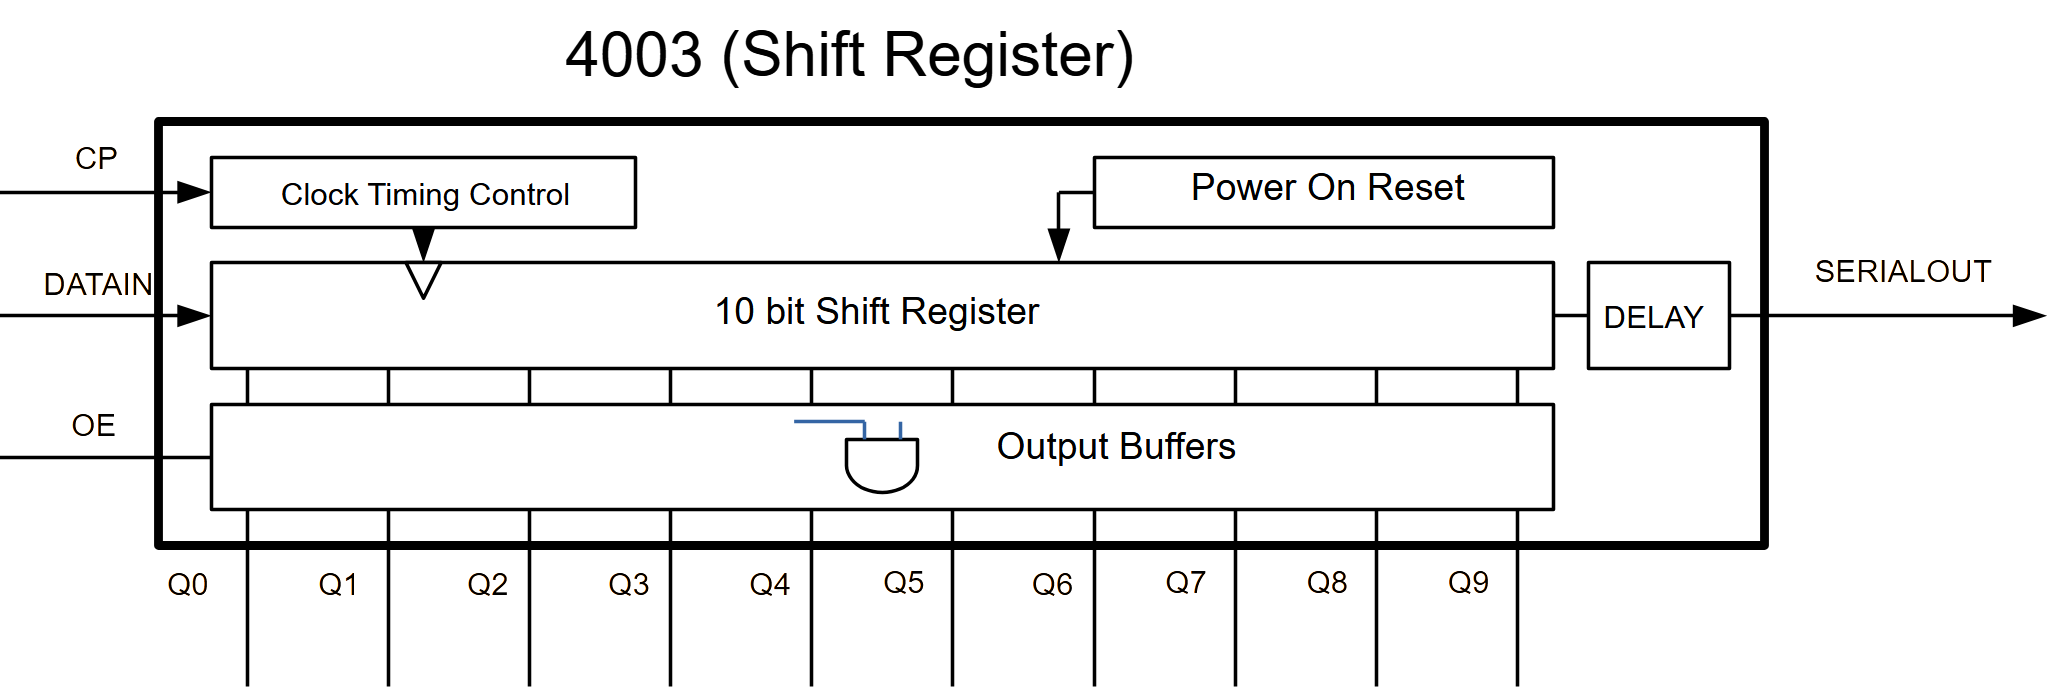
\includegraphics[width=1.0\columnwidth]{./Figure/Structure4003.png}
    \caption{Structure of 4003 Shift Register chip}
    \label{fig:STRUCTURE4003}
\end{figure}
%----------------------------------

%==============================================================
\section{MCS-4 System Configuration}
An example configuration of the MCS-4 system memory using the 4004 CPU, 4001 ROM, and 4002 RAM is shown in Figure \ref{fig:MCS4SYSTEM1}.  

This diagram illustrates the maximum system composition achieved by directly connecting each device to the CPU without any external circuitry.

It includes 16 ROM chips and 16 RAM chips spanning 4 banks.

%----------------------------------
\begin{figure}[h]
    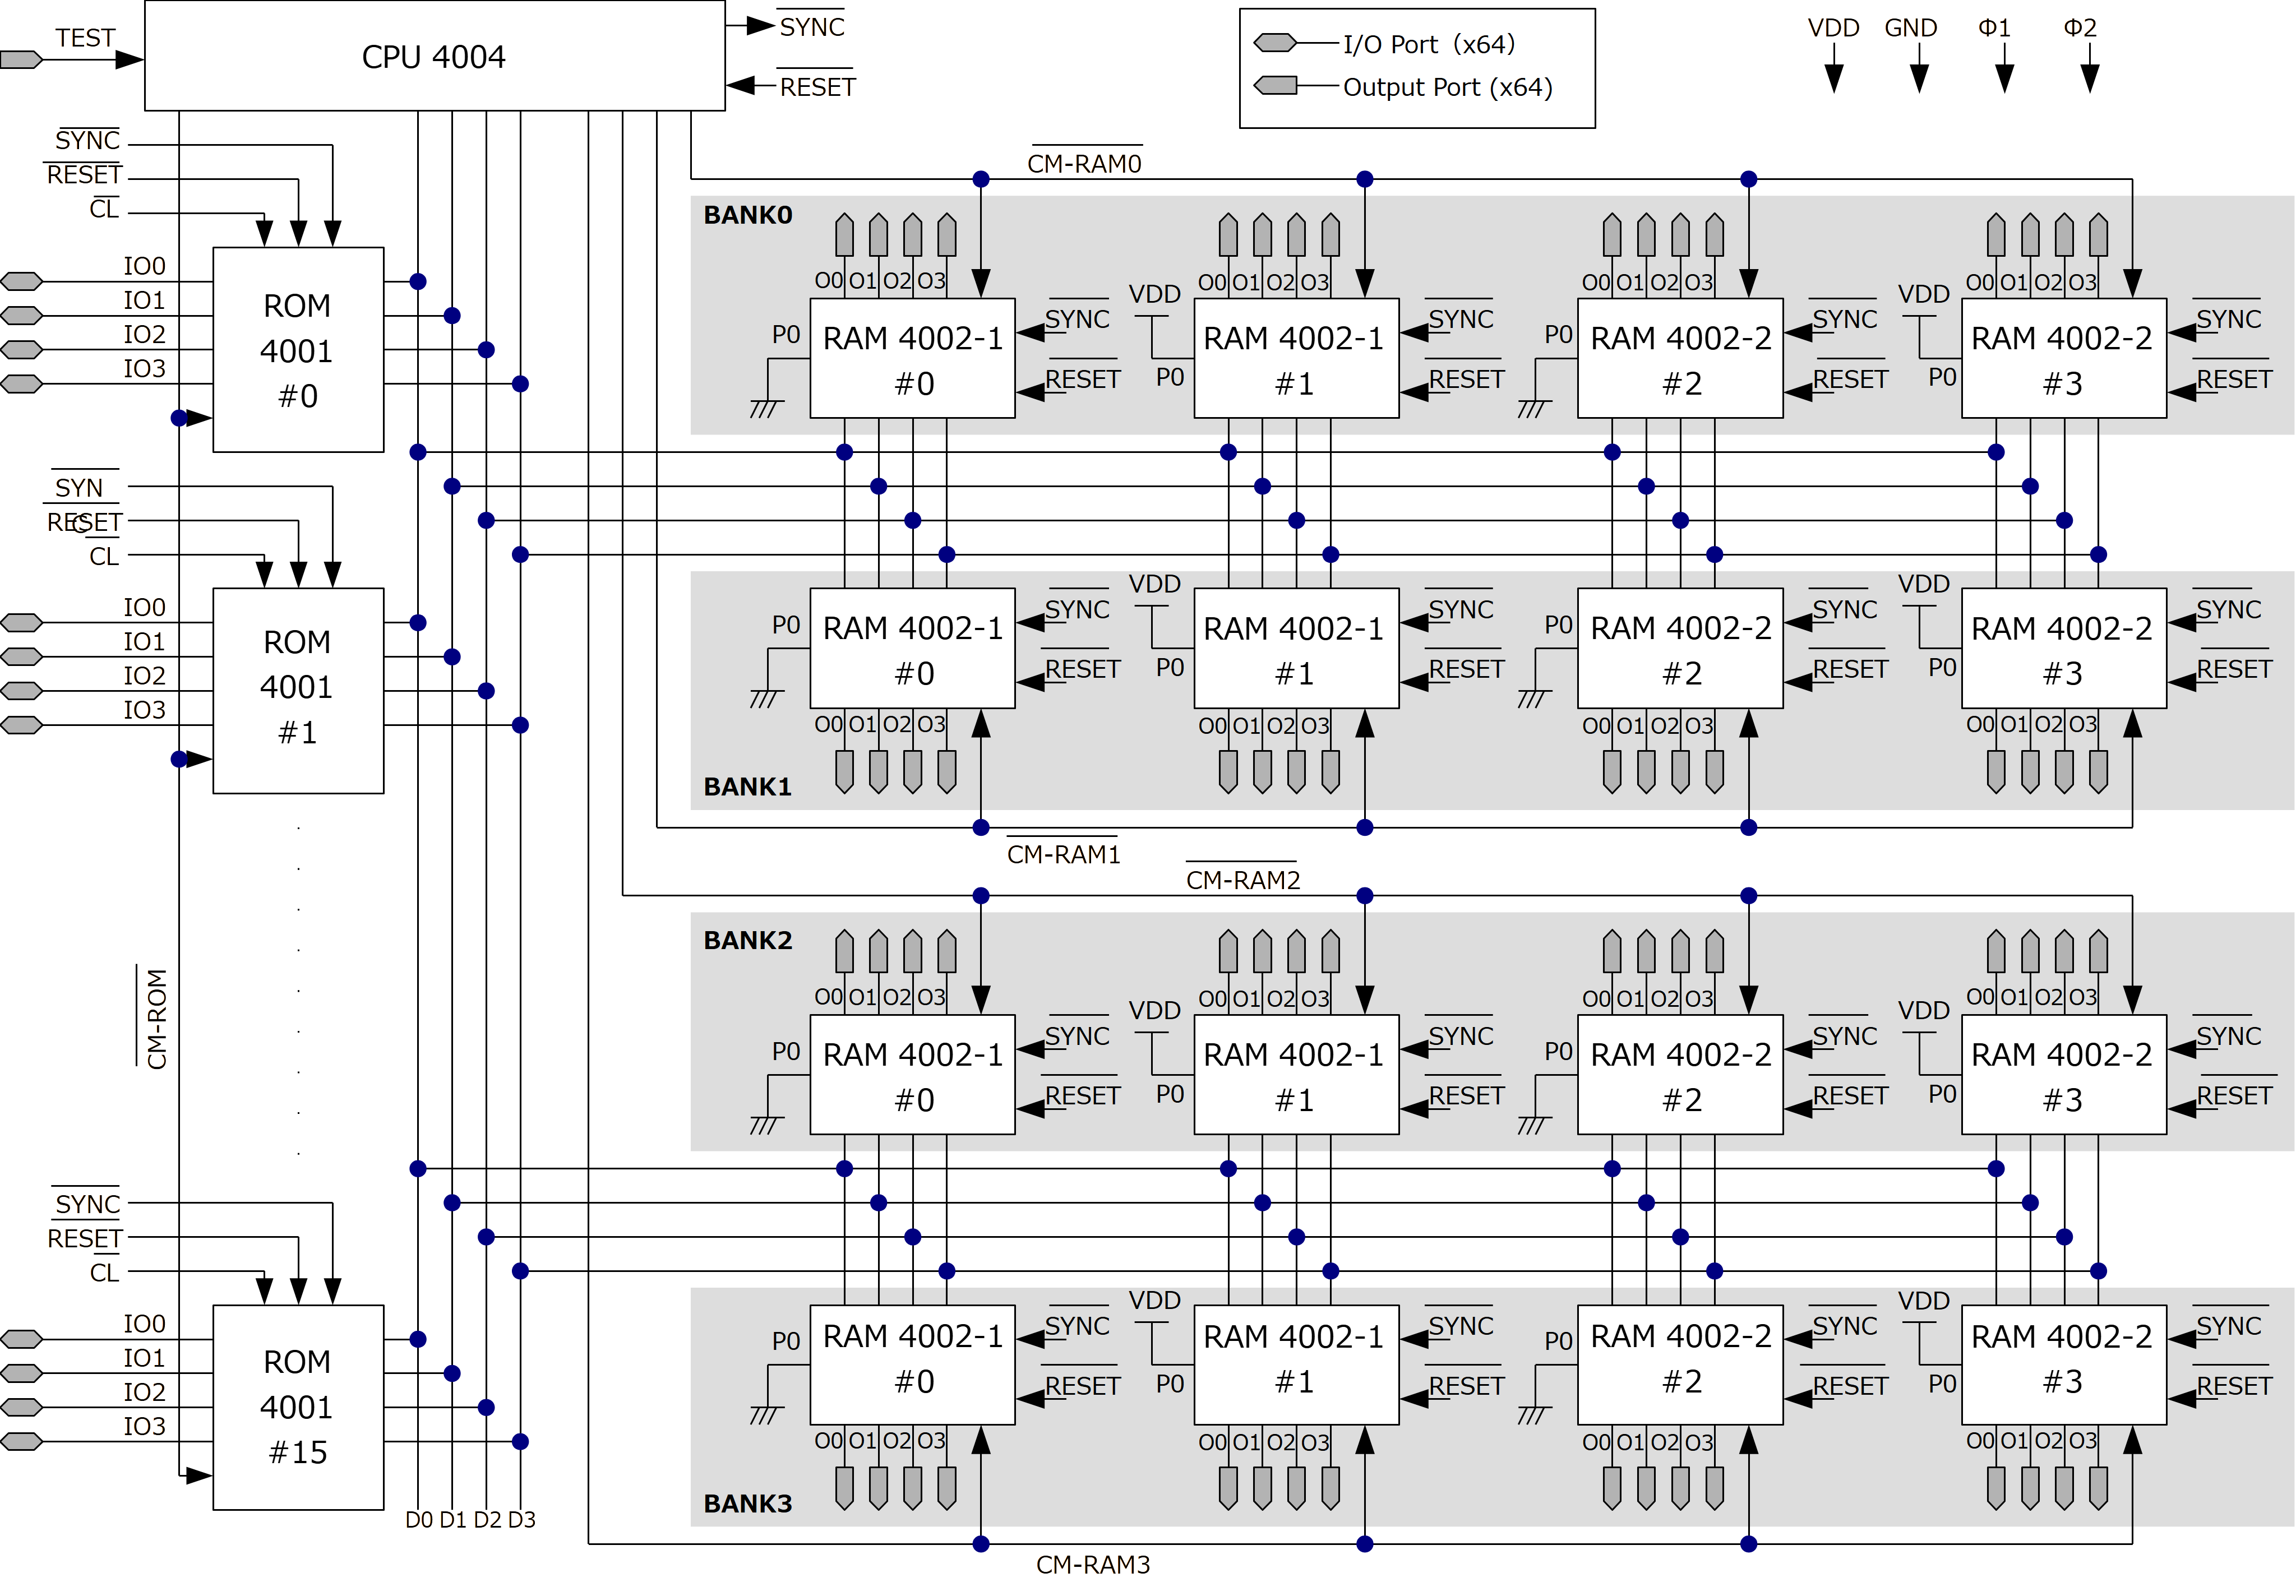
\includegraphics[width=1.0\columnwidth]{./Figure/MCS4System(1).png}
    \caption{Example Memory Configuration of the MCS-4 System}
    \textit{This diagram illustrates a configuration of the 4004 CPU along with the 4001 ROM and 4002 RAM, showcasing a maximum system built through direct connection of each device to the CPU.}
    \label{fig:MCS4SYSTEM1}
\end{figure}
%----------------------------------

%----------------------------------
\subsection{Is Something Missing?}
Carefully examine the system configuration in Figure \ref{fig:MCS4SYSTEM1}.  
Is there anything missing for it to be a complete microcomputer system?

As previously mentioned in the 4004 CPU pin description, the system lacks a dedicated address bus.
Instead, address information is transmitted via the 4-bit data bus using time-division multiplexing.

Beyond the absence of an address bus, consider other missing elements.  
For instance, the $\overline{\text{CM-ROM}}$ and $\overline{\text{CM-RAMx}}$ signals are fed into multiple ROM and RAM chips simultaneously.  
This suggests they cannot serve directly as individual chip select signals.

Additionally, there are no signals provided to designate read or write direction when accessing RAM or ports.  
Why is such a configuration still valid?

%----------------------------------
\subsection{Fundamental Concept of Data Access Method}
When the 4004 CPU accesses the ROM (I/O ports) or RAM (memory and output ports), it uses not a single instruction but a combination of instructions.

First, it executes an instruction to send address information, specifying the internal address of the target ROM or RAM chip.  
This address is stored internally, placing the addressed ROM or RAM in a ready state awaiting data access.

Next, the CPU executes a data access instruction.  
Data access instructions are prepared individually for each target and for each direction (read or write).

Here is the key point:  
When the CPU fetches a data access instruction, the ROM or RAM simultaneously monitors the fetched instruction.  
By doing so, they recognize what type of access the CPU intends to perform.  
During the execution states of the same instruction cycle, the targeted memory devices act accordingly, performing read or write operations via the data bus.

Thus, the system does not require explicit read/write direction signals—memory chips infer access direction by interpreting the instruction type itself.

Details about each instruction's behavior during actual data access will be explained in subsequent sections.

%----------------------------------
\subsection{Expansion of Output Ports in the MCS-4 System}
In the system configuration shown in Figure \ref{fig:MCS4SYSTEM1}, the 4001 ROM provides 64 I/O ports and the 4002 RAM offers 64 output ports.  

While this yields a substantial number of ports, such memory capacity is typically excessive for applications like calculators.

To ensure sufficient output port availability even with fewer ROM/RAM chips, a serial-to-parallel conversion IC was developed—the 4003 shift register.

Figure \ref{fig:MCS4SYSTEM1} illustrates an example of output port expansion using the 4003.  
In this setup, one standalone 4003 and two cascade-connected 4003 chips expand 6 output lines into 30 individual ports.

Although shift operation introduces latency before output stabilization, it remains effective for human interface and similar applications.

%----------------------------------
\begin{figure}[h]
    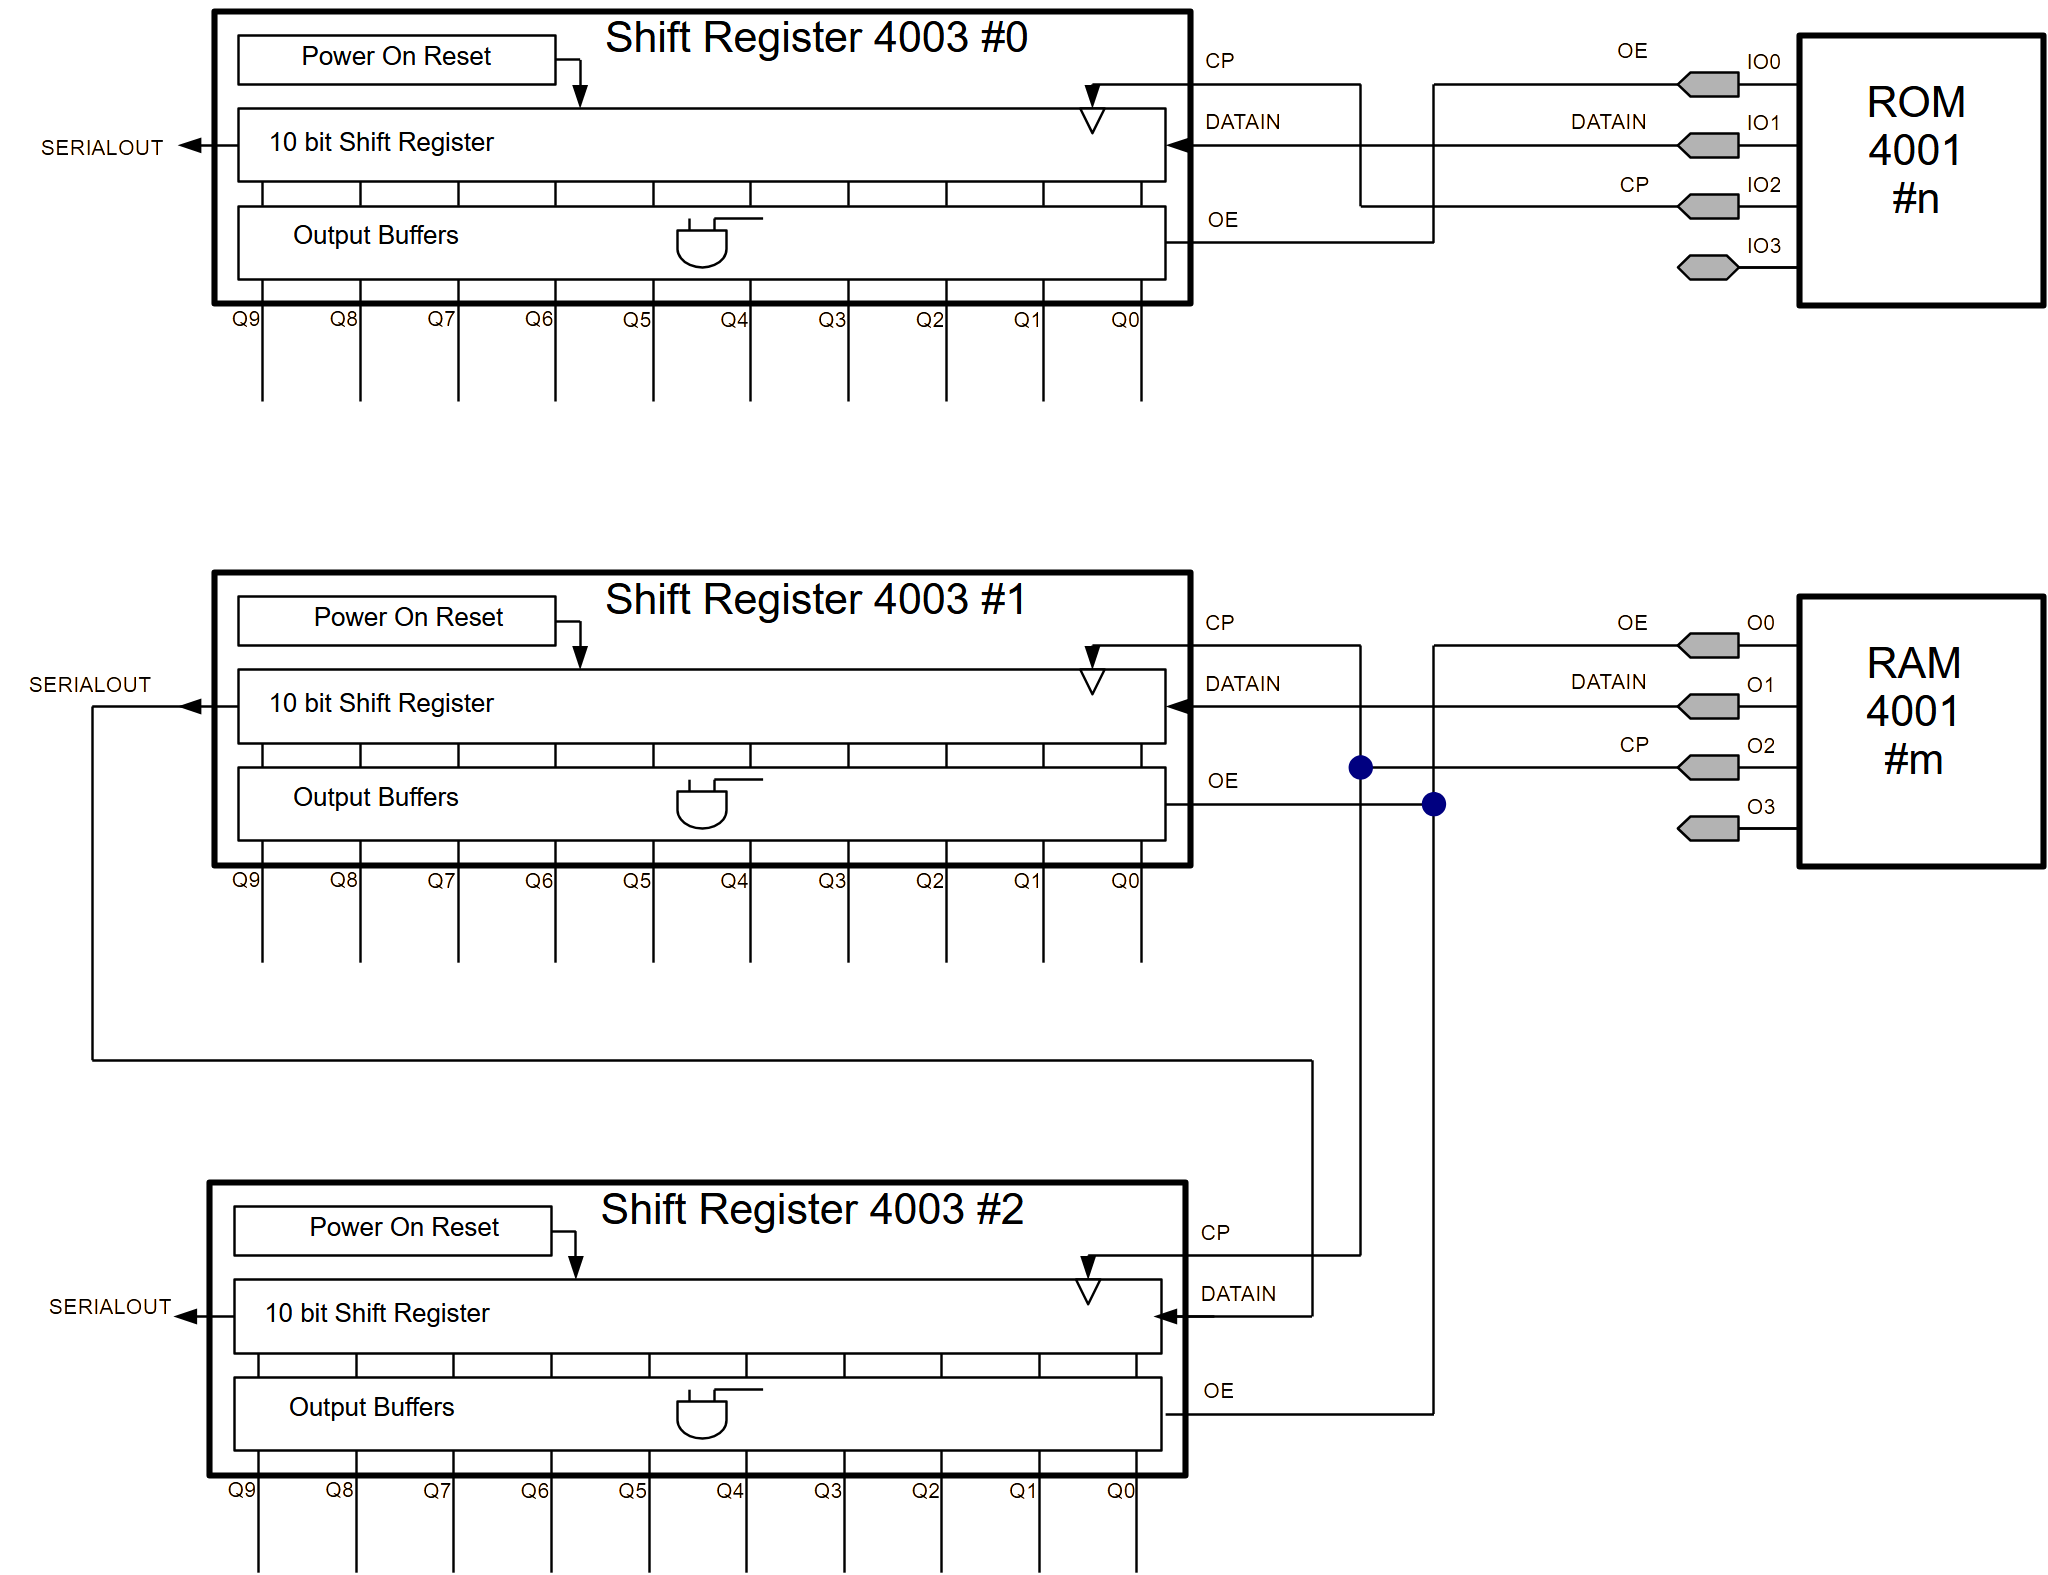
\includegraphics[width=1.0\columnwidth]{./Figure/MCS4System(2).png}
    \caption{Example MCS-4 System Configuration (2)}
    \textit{A wiring example showing how 4003 shift registers are connected to expand output ports.}
    \label{fig:MCS4SYSTEM2}
    \end{figure}
%----------------------------------

%==============================================================
\section{DC Characteristics of MCS-4 Chip Set}
%----------------------------------------------------
The actual MCS-4 chipset is manufactured using a 10~µm PMOS process. 

Its DC characteristics are shown in Table \ref{tb:DCCHARPMOS}.
The power supply voltage \texttt{VDD} is a negative potential relative to the ground reference \texttt{VSS}.

%----------------------------------------------------
\begin{table}[h]
\centering
\begin{tabular}{|l|c|c|c|c|l|}
\hline
\rowcolor{LightPurple}
\textbf{Item} & \textbf{Symbol} & \textbf{Min} & \textbf{Max} & \textbf{Unit} & \textbf{Remarks} \\
\hline
Power Supply & VDD & -15\,-5\% & -15\,+5\% & V &  \\
Low-Level Input Voltage & VIL & VDD & VSS\,-5.5 & V & Logic ``1'' level \\
Low-Level Output Voltage & VOL & VSS\,-12 & VSS\,-6.5 & V &  \\
High-Level Input Voltage & VIH & VSS\,-1.5 & VSS\,+0.3 & V & Logic ``0'' level \\
High-Level Output Voltage & VOH & VSS\,-0.5 & VSS & V &  \\
\hline
\end{tabular}
\caption{DC Characteristics of P-MOS Devices (MCS-4 Chipset)}
\label{tb:DCCHARPMOS}
\end{table}
%----------------------------------------------------

\paragraph{\textbf{Caution}}%
The MCS-4 system reproduced in this project is implemented on an FPGA. Under no circumstances should a \texttt{-15V} voltage be applied to the power supply or pins!

%==============================================================

